\documentclass{standalone}
\makeatletter\AtBeginDocument{\@buildstepset{1,2,3,4}}\makeatother
\usepackage{tikz}
\usetikzlibrary{intersections, calc}
\usepackage{hsbcommon}
\begin{document}
    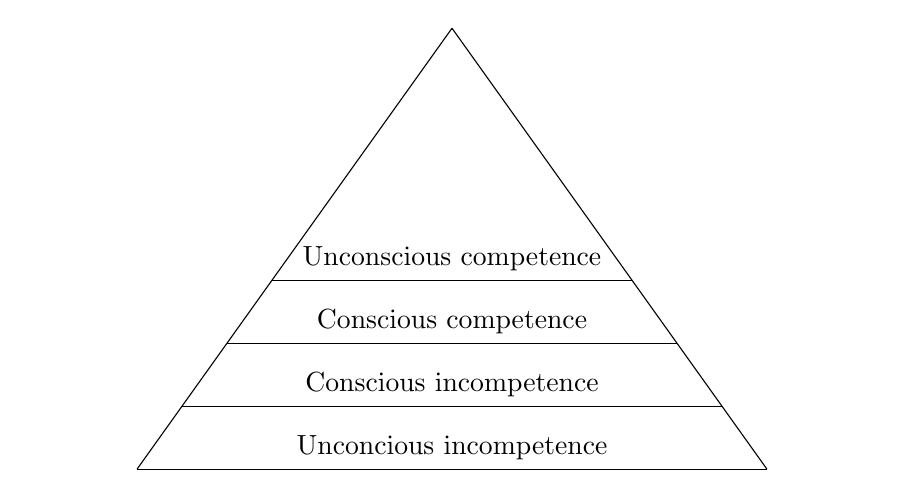
\begin{tikzpicture}[scale=0.8]
    \coordinate (A) at (-5,0) {};
    \coordinate (B) at ( 5,0) {};
    \coordinate (C) at (0,7) {};
    \draw[name path=AC] (A) -- (C);
    \draw[name path=BC] (B) -- (C);
    \foreach \y/\A in {
    0/Unconcious incompetence,
    1/Conscious incompetence,
    2/Conscious competence,
    3/Unconscious competence} {
        \path[name path=horiz] (A|-0,\y) -- (B|-0,\y);
        \draw[name intersections={of=AC and horiz,by=P},
              name intersections={of=BC and horiz,by=Q}] (P) -- (Q)
              node[midway,above,align=center,text width=
    \dimexpr(6em-\y em)*5\relax] {\A};
    }
    \end{tikzpicture}
\end{document}
